\section{Устройство акселерометра}

Акселерометр — прибор, измеряющий проекцию кажущегося ускорения (разности между истинным ускорением объекта и гравитационным ускорением) \cite{habr_mems}. Они широко применяются в смартфонах, автомобилях, промышленности и медицинских устройствах благодаря своей компактности, низкой стоимости и высокой точности.

МЭМС-акселерометр состоит из подвижной массы (инерционного элемента), закрепленной на упругих подвесах, и неподвижных электродов. При ускорении масса смещается, что приводит к изменению ёмкости или пьезоэлектрического сигнала, который преобразуется в электрический сигнал.

\begin{figure}[ht]
	\centering
	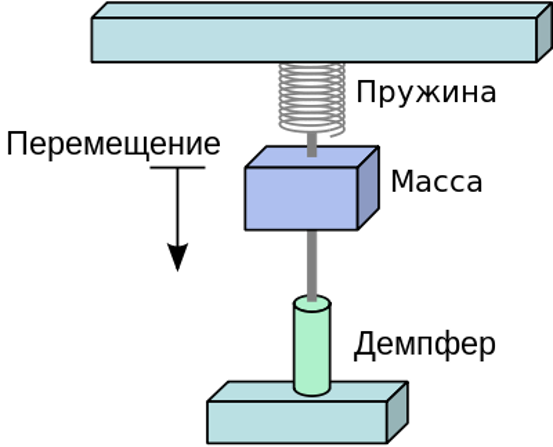
\includegraphics[width=0.5\textwidth]{images/theory/акселерометры/Схема работы акселерометра.png}
	\caption{Схема работы акселерометра}
\end{figure}

Основные методы измерения:

\begin{itemize}[label=$\circ$]
	\item Пьезоэлектрический
	\item Ёмкостный
	\item Тензорезисторный
\end{itemize}
\newpage